%!TEX root = ../thesis.tex
% This paragraph covered a lot of ground, but I was a bit lost since each sentence tried to cover too many different approaches. Is there an implied structure? E.g. first software-static, then software-video, then physical tasks? Id’ have expected some more basic references early on that for example show that people don’t read software documentation and instead look for task-centered learning materials. There’s also a difference between related work that investigates what good instruction formats are, and systems work that introduces new tools to create such formats.

\chapter{Background}
\label{chapter_background}

This dissertation proposes computational methods to create interactive tutorials for software applications and physical tasks. To ground our work in existing practices and principles, in this chapter, I define the terminology commonly used by tutorial researchers and online community (Section \ref{background_terms}).
%
I survey research studies and literature about the motivations of people creating, sharing, and consuming tutorials (Section \ref{background_why}) and a common creation process (Section \ref{background_creation}).
%
These insights are obtained from the following resources:
\begin{itemize}
  %\itemsep -2pt
  \item Formative studies from my research projects~\cite{Chi:2012:MAG:2380116.2380130,Chi:2014:DRS:2556288.2557254,Chi:2013:DGC:2501988.2502052}.
  \item Guidelines for creating instructions~\cite{InstructableHowTo,wikiHowHowTo}.
  \item An online survey of 2600 individuals across DIY communities~\cite{Kuznetsov:2010:REA:1868914.1868950}.
  \item Interviews of tutorial authorship and learning~\cite{Torrey:2007he,Torrey:2009fc,Wakkary:2015:TAH:2702123.2702550,Tseng:2014:PVP:2598510.2598540}.
  \item An analysis of 600 comments to web-based tutorials~\cite{BenLafreniere:2013ux}.
  \item Books of technical illustrations and expressing user experiences~\cite{mijksenaar1999open,greenberg2012sketching,Buxton:2007:SUE:1526229}.
\end{itemize}

% -------------------------------------------

\section{Instructions: Terminology}
\label{background_terms}

A \keyword{tutorial}, or a \keyword{how-to}, is a representation that transfers domain-specific \keyword{know-how} by describing a set of \keyword{instructions} on how to accomplish a specific task. Torrey \ea{} \cite{Torrey:2007he} defined:
\begin{quote}
\iquote{A How-To refers to online content that describes how something is done.}
\end{quote}
%
The title of a tutorial describes the goal of the task, such as \iquote{How to retouch photos with Photoshop} or \iquote{Create holiday photo cards.}
%
Instructions have been widely created for various domains, including:

\begin{itemize}
  %\itemsep -2pt
  \item Software applications, such as creating a motion blur effect of an image or creating a pie chart from a spreadsheet using specific software,
  \item Do-It-Yourself (DIY) projects, such as wrapping a gift box, assembling a piece of furniture, or building electronics with Arduino,
  \item Everyday activities, such as cooking or operating a vacuum machine, and
  \item Sports, such as making a dance move or swing a golf club.
\end{itemize}

Figure~\ref{fig:background_activities} shows example activities of these domains from online tutorials.
\\

\begin{figure*}[b!]
  \centering
  \begin{minipage}{\textwidth}
  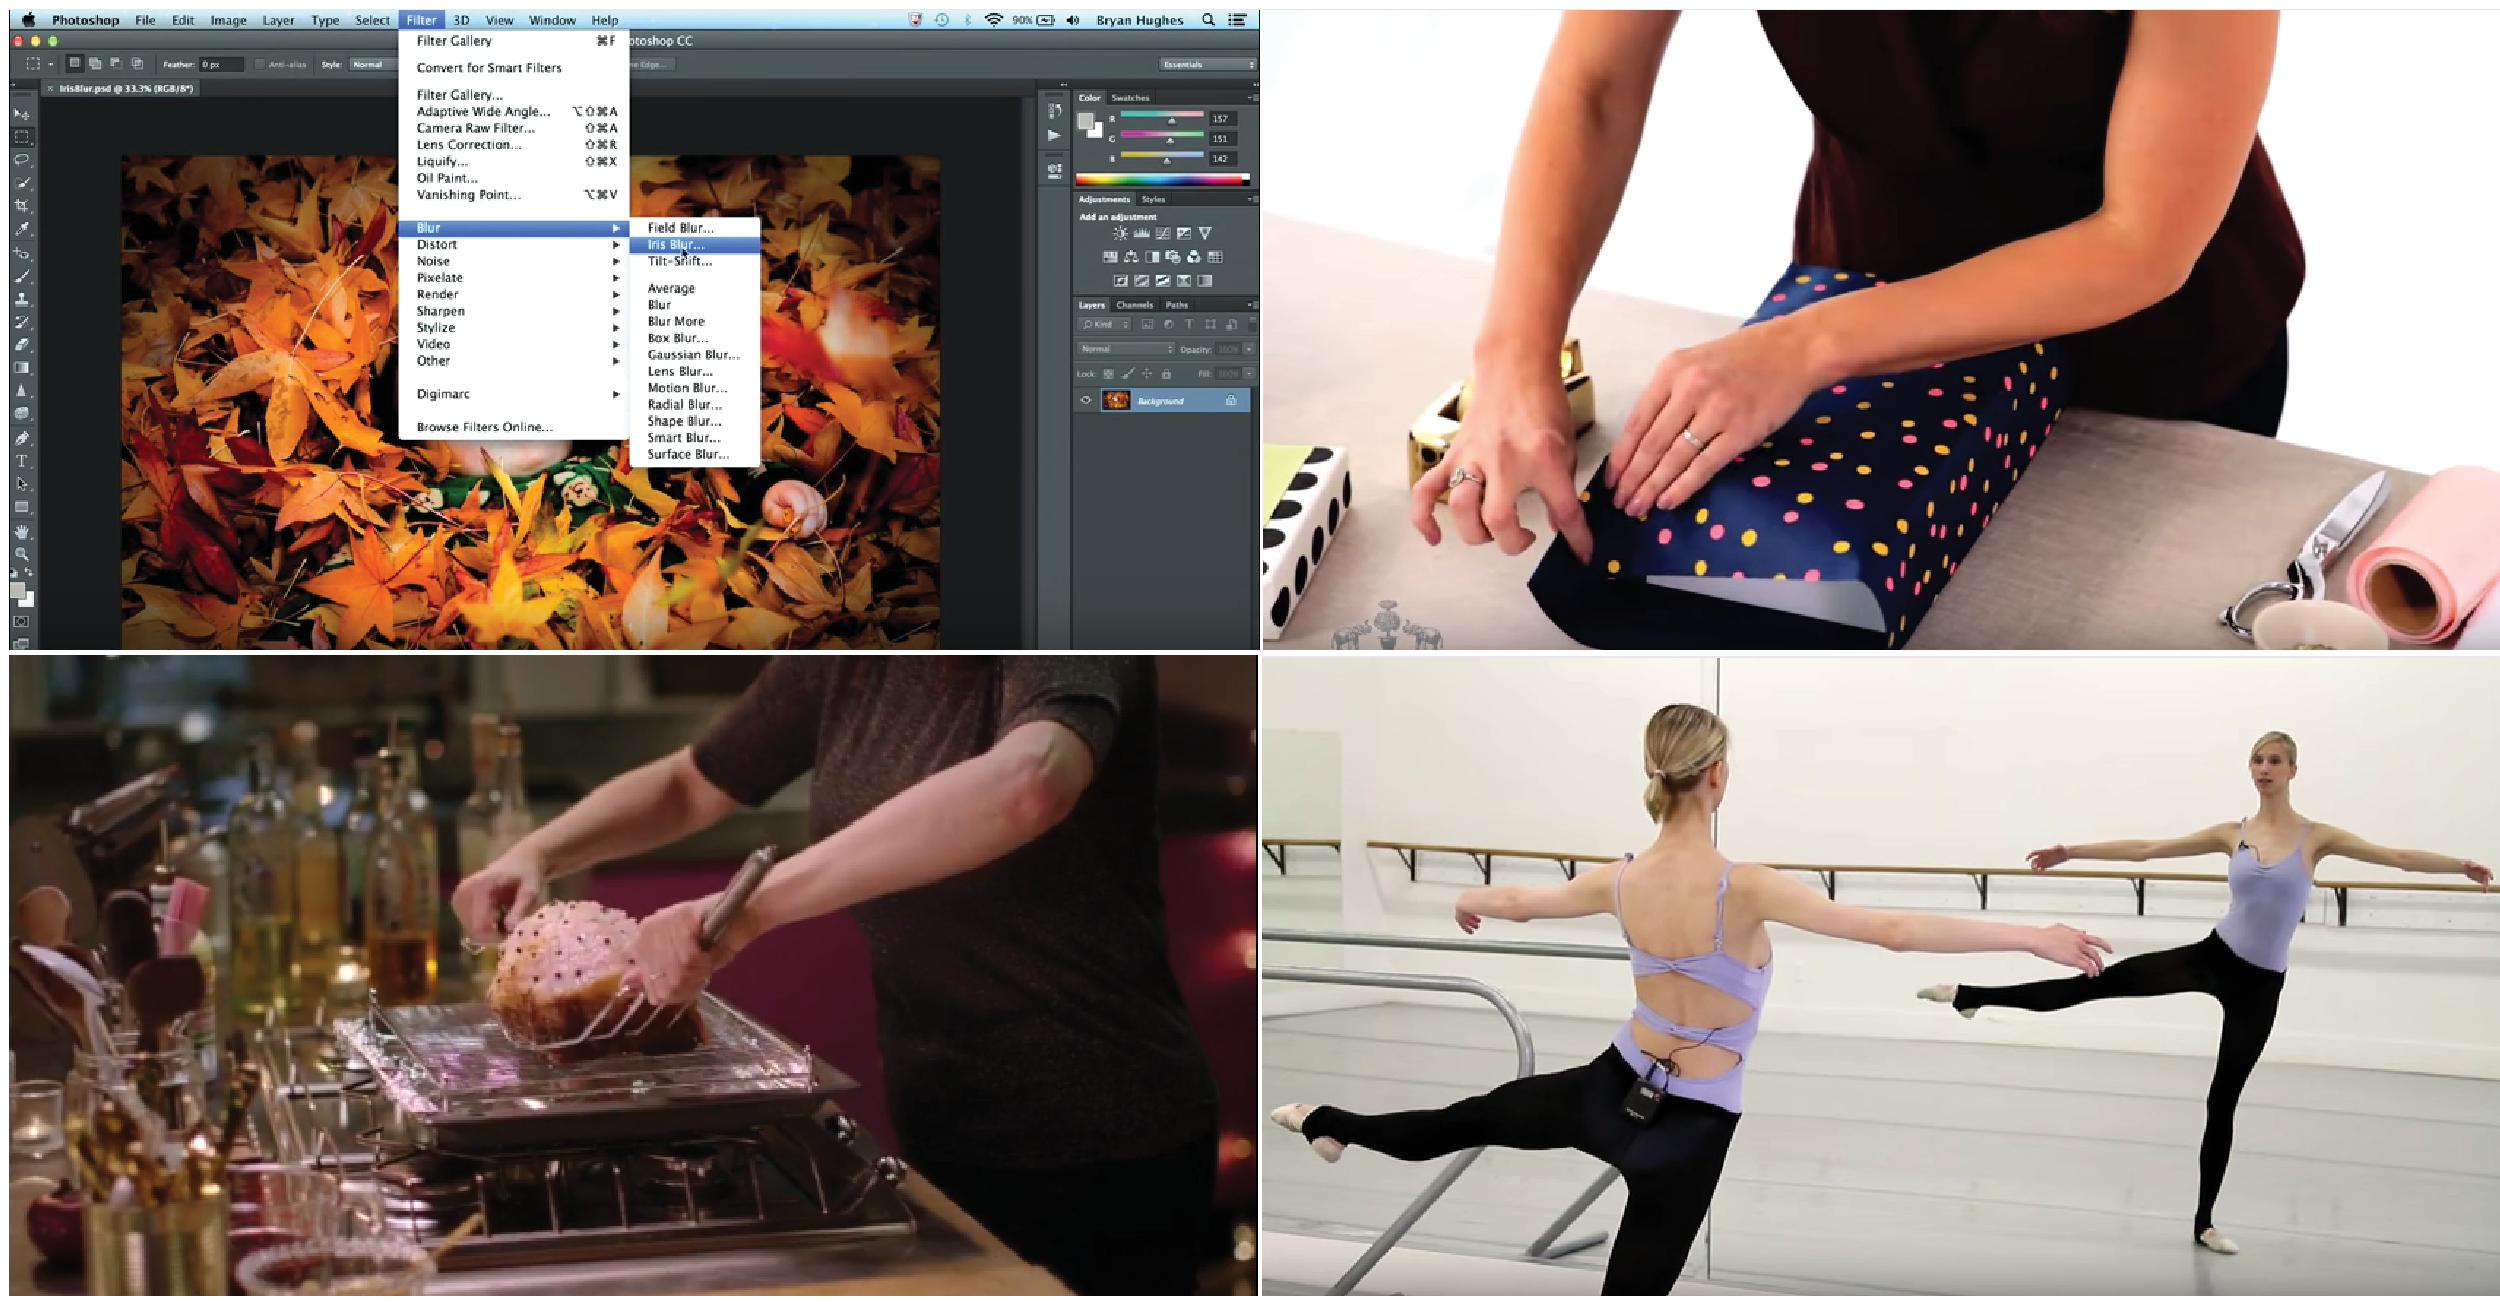
\includegraphics[width=\textwidth]{\background/fig/activities/activities}
  \caption[activities]{Example activities in tutorial domains:
  %
  a) image manipulations using a software application
  \footnote{Photoshop Playbook: Selective Focus, \url{https://youtu.be/Wh3ahxqDnyw}},
  %
  b) wrapping a gift, a DIY task
  \footnote{One Kings Lane: How to Wrap the Perfect Gift, \url{https://youtu.be/Me3ykrZobJE}},
  %
  c) cooking, an everyday activity
  \footnote{Slow-cooked black treacle ham, \url{http://www.bbc.co.uk/food/recipes/slow-cooked_black_21152}}, and
  %
  d) ballet dancing in sports
  \footnote{Ballet 101: How to Do the Fouette in Ballet Dancing, \url{https://youtu.be/DzqQNlaahjs}}.
  }
  \label{fig:background_activities}
  \end{minipage}
\end{figure*}

% A task-centric tutorial often involves domain-specific \keyword{know-how}, knowledge that is required to perform a task.
%
Instructional content is commonly structured as a list of \keyword{steps} or \keyword{subtasks} in a linear, \keyword{step-by-step} order.
%
It is important to include essential information required to complete a task, including materials, tools, preparation, expected outcome, and tips.
%
In some domains, instructions have been derived into specific formats. For example, cooking recipes contain not only actions but also food ingredients and required amounts.
% The term \keyword{recipe} has been used for activities other than cooking.

Note that instructions are different from a (software) \keyword{documentation}, \keyword{manual}, or \keyword{user guide}, which is a technical document contained non-task-centric details about a particular hardware or software system. A manual does not provide step-by-step guidance to follow. To accomplish a task, one needs to identify relevant information from the documentation and reason the workflow.

% -------------------

Instructions can be shown in different forms. There are two main forms of visual tutorials (see Figure~\ref{fig:background_formats}):
\begin{itemize}
  %\itemsep -2pt
  \item \keyword{Static tutorials}, which use text and figures to describe the set of operations required to accomplish a task. Such format is presented as a written document with a step-by-step list, while each step includes text description and/or an image or abstract illustration to describe the subtask. It can possible be combined into a \keyword{diagram} that shows the step procedure. Static tutorials are suitable for printing and are easy to scan because they show all instructions.
  \item \keyword{Video tutorials}, which are edited or raw videos of the tutorial author performing the task. Examples include screen recordings of a software application or a camera recording of a DIY task. Videos are effective to present the work in action, especially when the activities are hard to be described in text.
\end{itemize}

\begin{figure*}[th!]
  \centering
  \begin{minipage}{\textwidth}
  \includegraphics[width=\textwidth]{\background/fig/formats/formats}
  \caption[formats]{
    Major tutorial forms from online resources \footnote{Combine photos on the go, \url{https://helpx.adobe.com/mobile-apps/how-to/combine-photos-photoshop-mix.html}} \footnote{Change the color of an object, \url{https://helpx.adobe.com/photoshop/how-to/change-color-object-photoshop.html}}:
    %
    a) Step-by-step static tutorials show a list of steps, each with text and figure(s) that describe a subtask, such as \iquote{Start combining photos} or \iquote{Refine your composite}, and
    %
    b) video tutorials show an author performing the task, which can be reviewed and controlled via a video player.
  }
  \label{fig:background_formats}
  \end{minipage}
\end{figure*}

% -------------------

\subsection{Creating Instructions}
Instructions are created by one or more \keyword{authors} who document the process of completing a task and refine the material to a final deliverable.
%
Since the process often involves innovations and creations of the tasks of interests, authors can also be referred as \keyword{creators}, \keyword{makers}, or \keyword{hobbyists}.
%
Instructional authors are often the \keyword{professionals} or \keyword{experts} in the domains of their work. However, in tutorial production, they might be \keyword{amateurs} or \keyword{novices} who are not familiar with software tools to refine the documented material.

Throughout this dissertation, we call the process of author completing a task as a \keyword{demonstration} or a \keyword{performance}. Authors can therefore be as \keyword{demonstrators} or \keyword{presenters}.
%
In software, the demonstration process can be referred as a system \keyword{walkthrough}. Section \ref{background_creation} will discuss the production process of instructions.

% -------------------

\subsection{Consuming Instructions}
We define people who review instructional content as \keyword{viewers} or \keyword{learners}. Viewers may also be \keyword{followers} if they choose to follow the instructions in action to achieve the same or similar tasks.
%
Studies have shown that learners with different learning needs and habits have various preference on the tutorial formats. In Chapter \ref{chapter_mixt}, I'll examine these differences and propose a new instructional format.

% lecturer and online tutoring: involve more feedback collection and response to learners, beyond the scope of this paper

% -------------------------------------------

\section{Why Instructions?}
\label{background_why}

The research community has been investigating the motivations behind tutorial authors creating how-to videos and written instructions.
%
In early 90s, researchers studied users who formed online communities to collaboratively customize CAD systems \cite{Gantt:1992:GGP:142750.142767}. \iquote{Local experts} were found to play the key role within user groups. They provided supports to CAD system users of various levels of expertise by sharing customized environments and programmatic extensions. These experienced users were not professional programmers, but they were motivated by the frustrations of following manuals with existing software. They shared the materials in order to enhance manuals and help others acquire necessary skills.

The rise of maker movement from the 2000s introduced massive DIY project sharing via online services. Until mid-2016, Instructable has over 220,000 articles~\cite{InstructablesProjects}, and wikiHow provides 192,542 articles~\cite{wikiHowStatistics}.
%
Studies showed that one primary motivation of sharing DIY work is to demonstrate expertise ~\cite{Torrey:2007he,Kuznetsov:2010:REA:1868914.1868950}. Specifically, of the online survey that Kuznetsov and Paulos~\cite{Kuznetsov:2010:REA:1868914.1868950} conducted in 2010, 97\% of their 2608 respondents shared and contributed to projects to \iquote{Express myself/be creative.} Published tutorials serve as a way to broadcast skill and as an online portfolio.
%
Authors may derive revenue through advertising or referrals~\cite{Lafreniere:2012tl}, which was similar to how local, non-professional experts gained formal supports in CAD communities that Gantt \ea{}~\cite{Gantt:1992:GGP:142750.142767} found.

Viewers, on the other hand, typically seek technical explanations, but are also searching for inspiration~\cite{Torrey:2009fc} and looking for validation of existing skills~\cite{Lafreniere:2012tl}.
%
It was shown that people prefer web-based tutorials over manual as they provide \iquote{an immediate, specific goal to accomplish} and can help learners \iquote{shadow and experience an expert's work practices}~\cite{BenLafreniere:2013ux}.

While these studies present motivations beyond broadcasting and consuming instructions, research also found that creating ready-to-publish content can be time-consuming ~\cite{Kuznetsov:2010:REA:1868914.1868950}. Next, I discuss current practices of a tutorial production process.

% Make channel: 1,229,404 subscribers • 253,518,445 views
% Joined Mar 22, 2006
% https://www.youtube.com/user/makemagazine
% June 19, 2016
% \cite{MakerMediaKit}

% -------------------------------------------

\section{Techniques of Effective Instructions}
\label{background_techniques}

[To add: discuss existing practices]

\subsection{Annotated Diagrams}

~\cite{mijksenaar1999open}
Arrows
movements, speed,

Pictorial
call-outs, highlights (color, rectangle, circle, bubbles)
attention, warnings

https://youtu.be/Wv7sdHEdaR0?t=1m41s

Text
descriptive

Sequences
numbers, layout, arrows

\subsection{Instructional Videos}

DemoCut: cuts, zoom, transitions, subtitles, auditory effects

above techniques from annotated diagrams are often seen: arrows, call-outs, text,...

\begin{figure*}[t!]
  \centering
  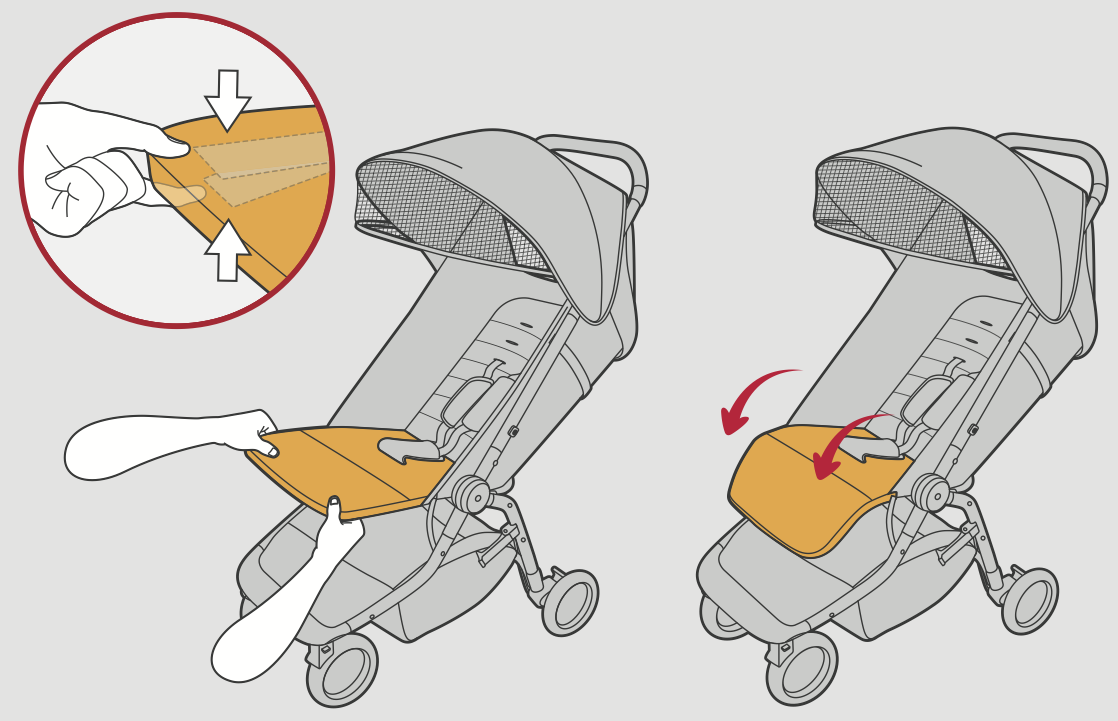
\includegraphics[width=0.7\textwidth]{\background/fig/illustration/illustration}
  \caption{\tofix{discuss techniques here}}
  \label{fig:background_techniques}
\end{figure*}

% -------------------------------------------

\section{Instruction Production Process}
\label{background_creation}

\begin{quote}
\iquote{The practice of writing and sharing DIY tutorials is at the heart of the distributed production and creativity of DIY. Tutorials not only provide tutorship of particular projects, they also develop the skills and competences of those involved in DIY and, in doing so, expand the culture and practices of DIY. It is fair to say that the vitality of DIY practices relies on the effectiveness and quality of tutorials.} -- Wakkary \ea{}~\cite{Wakkary:2015:TAH:2702123.2702550}
\end{quote}

In their paper discussing tutorial authorship, Wakkary \ea{}~\cite{Wakkary:2015:TAH:2702123.2702550} pointed out the values of producing DIY tutorials, which I believe can be applied to instructions of other domains. However, the time required to create a tutorial is the primary concern for authors~\cite{Kuznetsov:2010:REA:1868914.1868950}, especially for activities that involve more steps, tools, and material. To produce a tutorial, an author may go through several stages:
% Key findings include identifying tools and components and structuring a task into steps with a clear sequence.

Torrey \ea{}~\cite{Torrey:2007he} proposed a project lifecycle of three phases: 1) the ``project'', which is a goal or a challenge to achieve, 2) the ``story'' by documenting the making via words and text, and 3) the ``contribution'', which is to broadcast the How-To.
%
Tseng and Resnick~\cite{Tseng:2014:PVP:2598510.2598540} found that ``documenting'' and ``designing'' a DIY project are often separate processes.
%
Our interviews with instructional authors on YouTube suggested that a production process can be similar to a filming production~\cite{Chi:2013:DGC:2501988.2502052}.
%
Figure~\ref{fig:background_creation} shows a typical tutorial creation workflow that we identified, which includes four main stages: \iquote{planning} a procedure of achieving the goal of a task or a project, \iquote{capturing} the process of completing the project, \iquote{editing} the captured material into a form that can be followed, and finally \iquote{sharing} the instructions to the communities.
%
Some tutorial creators, especially professionals, may work as a team with multiple role players in a production process, while some work individually. The time required to create a tutorial may vary from a few minutes to weeks.

Below I describe the characteristics of each stage in detail.

\begin{figure*}[t!]
  \centering
  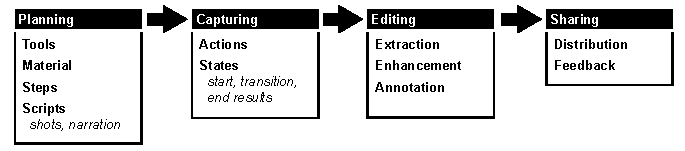
\includegraphics[width=\textwidth]{\background/fig/creation_process}
  \caption{A common workflow of tutorial creation, which includes planning the task in detail, capturing the process, editing the captured material into a readable form, and sharing with the communities.}
  \label{fig:background_creation}
\end{figure*}

% ------------------------

\subsection{Planning}
Planning or preparation helps authors gather ideas, inspirations, and necessary details prior to building a tutorial project~\cite{Torrey:2007he}. At this stage, authors decide the project scope and expected outcome, confirm the material and tools required, and design subtasks or steps to be executed. Some authors choose to explicitly write detailed scripts to explain their activities during the capturing stage~\cite{Chi:2013:DGC:2501988.2502052}. Figure~\ref{fig:background_scripts} presents examples of instructional video scripts.

\begin{figure*}[th!]
  \centering
  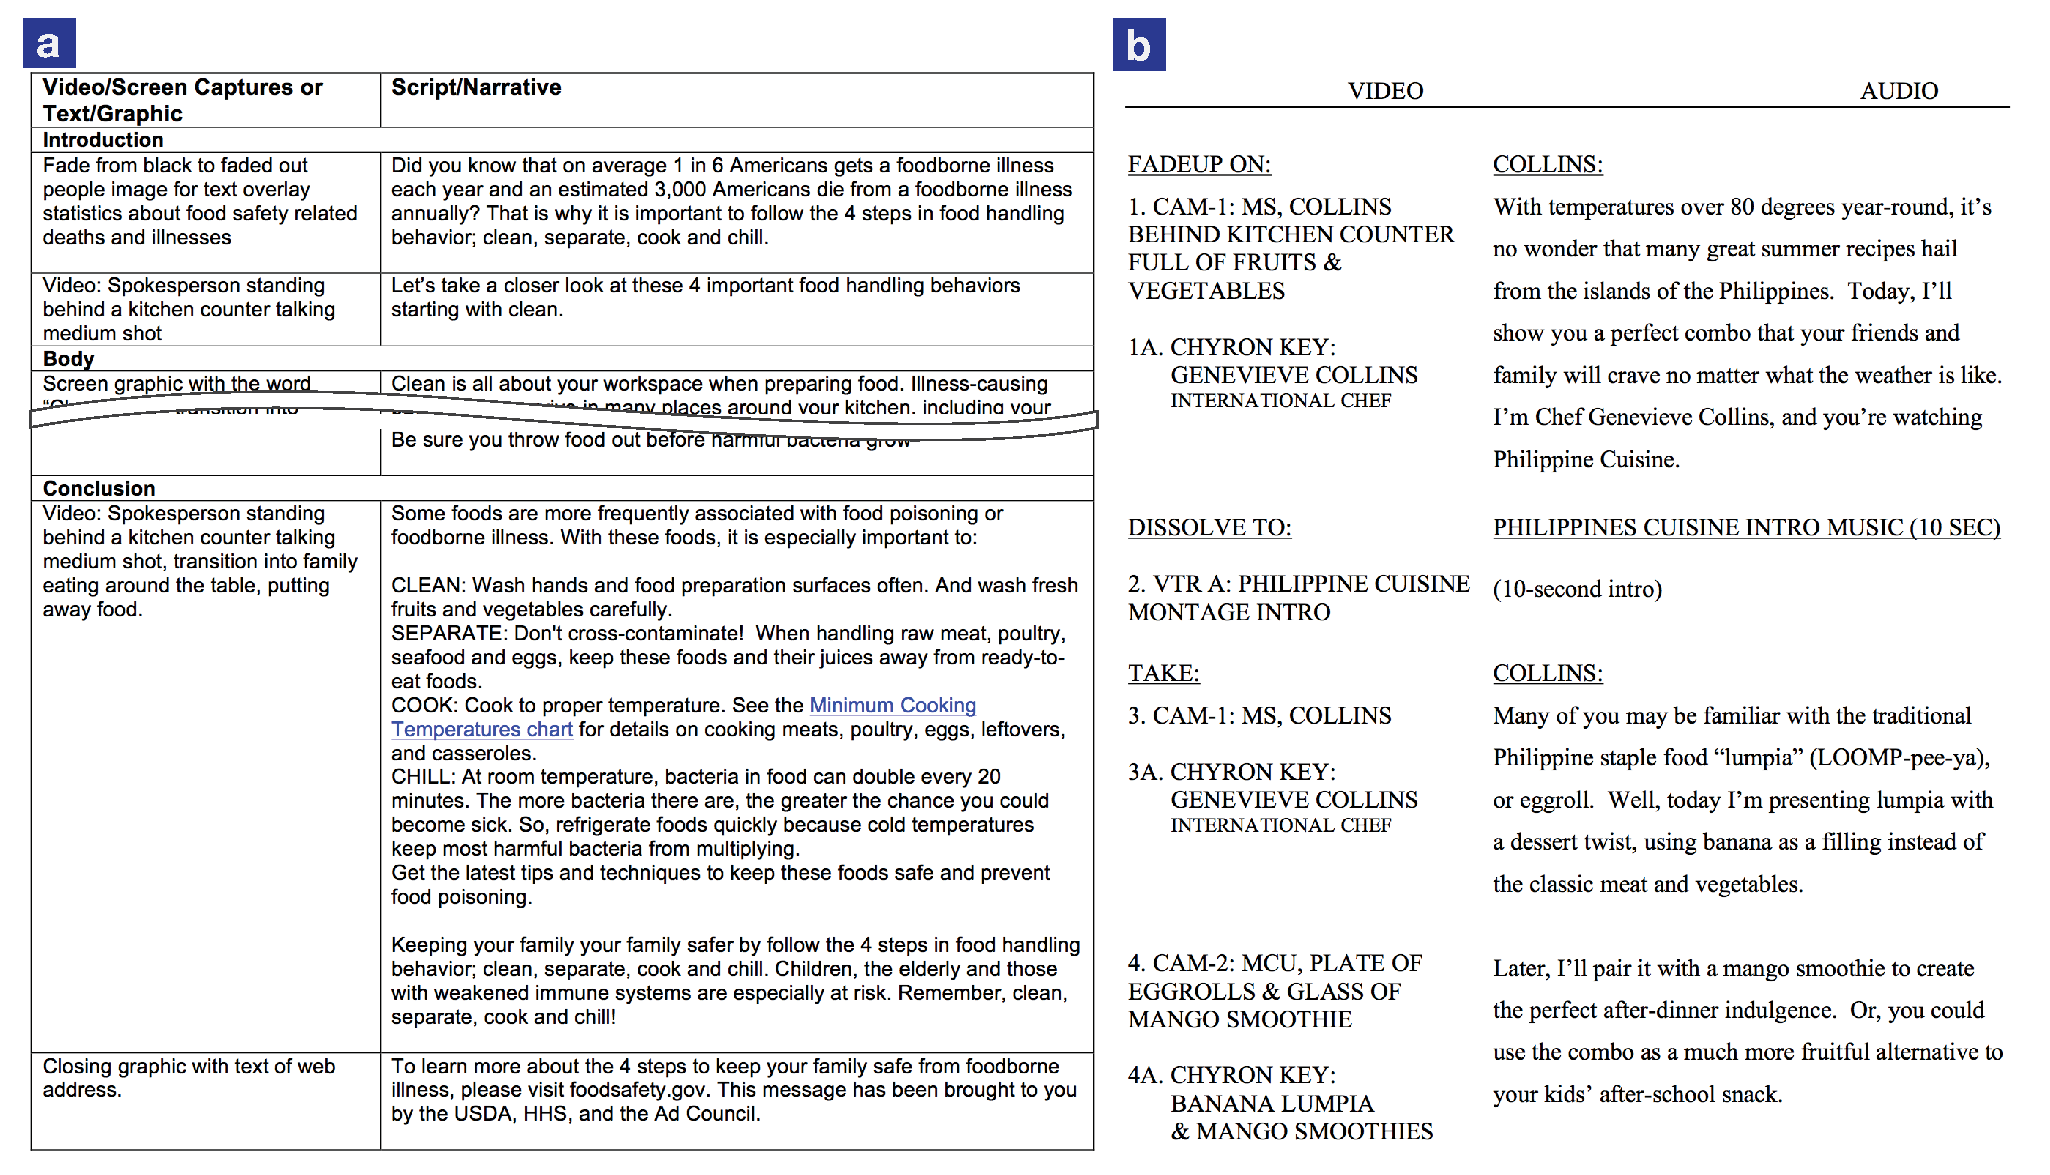
\includegraphics[width=\textwidth]{\background/fig/scripts/scripts}
  \caption{Example scripts for instructional videos about a) food safety~\protect\cite{WisconsinFoodSafetyScript} and b) cooking ~\protect\cite{SouthernIllinoisScript}. Each includes video shot(s) and narration, some with additional notes on the actions. High-level structure can also be specified, such as ``introduction'' and ``conclusion.''}
  \label{fig:background_scripts}
\end{figure*}

\subsection{Capturing}
Documenting or capturing is the core of creating instructions in order to guide viewers through a specific task. At this stage, authors document the process of task demonstration via recording devices, such as digital cameras, camcorders, and mobile devices. They capture necessary actions using tools and materials, as well as the changing of states of the elements. %(e.g., how )
%
Mutlimedia material has been found to be effective to document procedural knowledge~\cite{Kuznetsov:2010:REA:1868914.1868950,Wakkary:2015:TAH:2702123.2702550}, including:

\begin{itemize}
  \item Static photographs that capture specific moments in a procedure.
  \item Video footages that record a computer screencast or a scene of a demonstration.
  \item Audio recordings that preserve the sound of activities or author narration. The narration can be transcribed into text for reading.
  \item Other domain-specific content (e.g., code, circuit board layouts, 3D models, and sketches) or resources (e.g., books or URLs to other material), which often serve as supplementary material.
\end{itemize}

\subsection{Editing}
After collecting necessary material, the majority of efforts and time often devotes to editing--to turn the raw material in a concise form.
Photographs need to be cropped and resized~\cite{Tseng:2014:PVP:2598510.2598540}, sometimes annotated~\cite{Torrey:2007he}; videos require removing footage, applying visual effects and transitions; audio has to be processed to omit utterances and condense narration~\cite{Chi:2013:DGC:2501988.2502052}. Popular editing tools include Adobe Photoshop and Apple Final Cut Pro, and emerging mobile applications such as Snapguide have been adopted by novices.

Different multimedia forms can be mixed to create tutorial formats mentioned in Section~\ref{background_terms}. Videos, in particular, have become a popular medium to document and demonstrate the functionality of the work:

\begin{quote}
\iquote{Videos, for instance, require a long time to edit, but can influence the viewer in at least three powerful ways: 1) by physically illustrating the steps required to create an artifact; 2) by showcasing a new idea in its functional form; and 3) by directly `speaking' to and engaging with the audience.} -- Kuznetsov and Paulos~\cite{Kuznetsov:2010:REA:1868914.1868950}
\end{quote}

\subsection{Sharing}
Finally, authors may release the refined content and share the deliverable with others. Common media or platforms include: personal blogs, content sharing sites, forums, emails, or personal networks.
%
Some of these channels offer ways for the audience to provide feedback and contribute. Lafreniere \ea{}~\cite{Lafreniere:2012tl} specifically analyzed the online comments to web tutorials. Their study shows that the audience has several purposes to communicate via comments, including technical validation and refinement, which can be useful for authors to improve their documentation techniques.

% , depending on the stages involved and the content.

% -------------------------------------------

\section{Summary}

These studies and observations suggest that tutorials have a larger variety of purposes and uses than merely communicating technical content.
%
In my dissertation, I strive to make authoring of instructions more accessible to amateurs while maintaining opportunities for adding individual style through control over editing effects.
%
Next, I survey prior work on computational methods of supporting authoring and following instructions.
